\chapter{Практические приложения}
\label{cha:applications}

В этой главе мы рассматриваем роль сингулярных элементов модулей аффинных алгебр Ли в приложениях к задачам конформной теории поля. Мы используем установленные в главах \ref{cha:affine-lie-algebras}, \ref{cha:BGG}, \ref{cha:splints} свойства для эффективных вычислений. 

\section{Coset-модели и критическое поведение}

% и  Эволюция Шрамма-Левнера и алгебраические свойства предельного перехода от решеточных моделей к конформной теории поля}
\label{sec:SLE}

Алгебраические методы в конформной теории поля позволяют получать явные уравнения на корреляционные функции (например, уравнения Книжника-Замолодчикова \eqref{eq:66} в ВЗНВ-моделях и их аналоги в coset-моделях \eqref{eq:101}). Во многих случаях эти уравнения можно решить аналитически либо численно и получить конкретные значения для физических величин, например, для критических индексов. Таким образом конформная теория поля является мощным инструментом для описания критического поведения в решеточных моделях. 

Однако соответствие между решеточными моделями и конформной теорией поля, описывающей их критическое поведение, не так легко установить. В случае простых моделей (Изинга, Поттса, Ашкина-Теллера и т.д.) и минимальных моделей конформной теории поля такое соответствие первоначально устанавливалось путем сравнения центральных зарядов и конформных размерностей. Но соответствие корреляторов нуждается в строгом доказательстве. Один из инструментов изучения решеточных моделей -- эволюция Шрамма-Левнера -- позволяет в некоторых случаях доказать такое соответствие (см. \cite{duminil2011conformal,chelkak2009universality,smirnov2007towards,smirnov2001critical,Cardy:2005kh,bauer2004conformal,bauer2004sle,bauer2004cfts,bauer2003sle,friedrich2003conformal,bauer2002sle}). Класс моделей конформной теории поля, для которых получены такие результаты, в основном ограничивается минимальными унитарными моделями. 

Эволюция Шрамма-Левнера -- это стохастический процесс, который предложил Oded Schramm  \cite{schramm2000scaling} для описания скейлингового предела критических интерфейсов в двумерных статистических решеточных моделях. Этот подход к критическим системам дал много строгих результатов в теории критического поведения (см. обзоры  \cite{rohde2005basic}, \cite{bauer20062d}, \cite{Cardy:2005kh}). В разделе \ref{sec:schr-loewn-evol} мы приводим необходимые определения.  

Вероятностная мера, порожденная эволюцией Шрамма-Левнера на случайных кривых, конформно-инвариантна. Так как конформная теория поля представляет собой другой метод для изучения двумерных критических систем, естественно изучать ее связь с эволюцией Шрамма-Левнера. Такая связь изучалась, например, в работах \cite{bauer2004conformal,bauer2004cfts,bauer2003sle,bauer2002sle} (и многих других), но в основном для минимальных унитарных моделей. 
Идея состоит в рассмотрении определенных наблюдаемых в области с разрезом. Эта конструкция обсуждается в разделе \ref{sec:corr-betw-sle}. 

Как мы показали в главе \ref{cha:CFT}, более общие модели конформной теории поля обладают дополнительными симметриями. Так в моделях Весса-Зумино-Новикова-Виттена и в coset-моделях возникают аффинные алгебры Ли.  Чтобы реализовать эти симметрии при изучении эволюции Шрамма-Левнера, нужно ввести дополнительное случайное блуждание на группе Ли \cite{bettelheim2005stochastic}, \cite{Rasmussen:2004xr}. Такое случайное блуждание определяется в разделе \ref{sec:sle-wzw-models}. Соответствие между мартингалами эволюции Шрамма-Левнера и корреляционными функциями в моделях Весса-Зумино-Новикова-Виттена изучалось в работе \cite{alekseev2010sle}. Аналогичное обобщение на $\mathbb{Z}(N)$-парафермионную модель было предложено в статьях \cite{santachiara2008sle,picco2008numerical}. 

Мы обобщаем эволюцию Шрамма-Левнера с дополнительным случайным блужданием на группе Ли на случай фактор-пространства  $G/A$ и в изучении связи с coset-конструкцией конформной теории поля. По аналогии со случаем моделей Весса-Зумино-Новикова-Виттена мы получаем систему алгебраических уравнений на оператор смены граничного условия из условия на мартингал. 
При помощи coset-конструкции можно реализовать минимальные и парафермионные модели конформной теории поля (см. \cite{difrancesco1997cft}).  Мы сравниваем наши уравнения на оператор смены граничных условий с результатами работы \cite{santachiara2008sle} и видим, что они совпадают. Кроме того, полученные нами значения параметров эволюции Шрамма-Лёвнера согласуются с результатами для минимальных моделей.

%%  В разделе  \ref{sec:5-conclusion} мы обсуждаем возможность сравнения классификации операторов смены граничных условий, следующей из свойства мартингалов с общей классификацией операторов смены граничных условий в граничной конформной теории поля, связанной с D-бранными решениями \cite{fuchs2005geometry,fredenhagen2002d,elitzur2002d,Maldacena:2001ky,felder1999geometry,alekseev1999d}. 
%%  

\subsection{Эволюция Шрамма-Левнера}
\label{sec:schr-loewn-evol}
Рассмотрим модель Изинга на треугольной решетке в верхней полуплоскости (см. Рисунок \ref{fig:sle}). Наложим следующее граничное условие: потребуем, чтобы на одной половине границы все спины были направлены вверх, а на другой половине -- вниз. Тогда при любой конфигурации спинов на полуплоскости будет интерфейс, разделяющий два кластера и соединяющий точку ноль с бесконечностью (см. Рисунок \ref{fig:sle}).

\begin{figure}[h]
  \centering{
    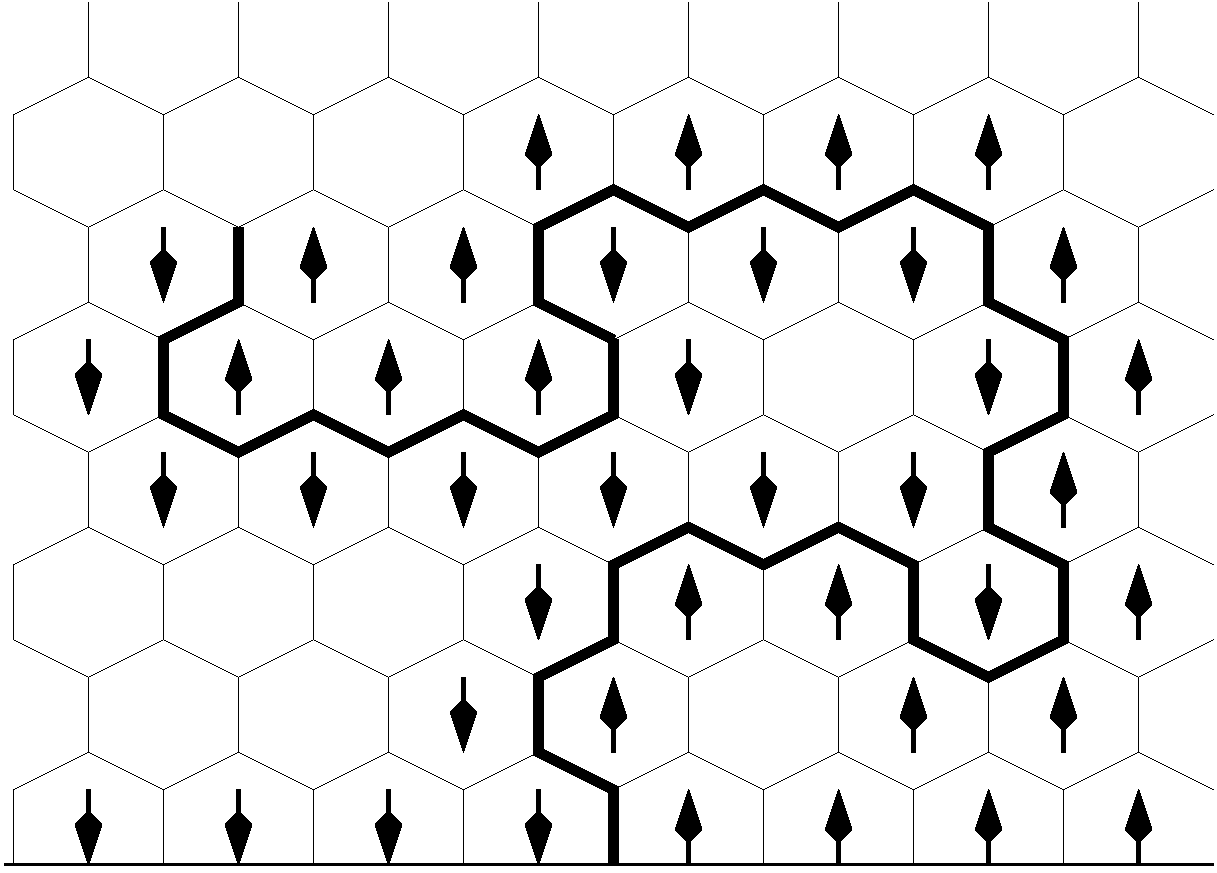
\includegraphics[height=50mm]{explore}
    \caption{Интерфейс в модели Изинга на треугольной решетке}}
  \label{fig:sle}
\end{figure}
Мы можем наложить условие существования части интерфейса конечной длины и рассмотреть конфигурации статистической модели, удовлетворяющие этому условию. Очевидно, такие конфигурации эквивалентны конфигурациям модели на области с разрезом вдоль интерфейса. 

Теперь рассмотрим непрерывный предел решеточной модели с (частью) интерфейса конечной длины. Интерфейсы в случайных конфигурациях модели сходятся к случайной кривой. Старая гипотеза \cite{Polyakov:1970xd} о конформной инвариантности в критической точке была недавно строго доказана для некоторых решеточных моделей (см. \cite{smirnov2007towards}, \cite{duminil2011conformal}). Мы предполагаем наличие конформной инвариантности в критической точке и рассматриваем верхнюю полуплоскость  $\mathbb{H}$ с разрезом вдоль критического интерфейса  $\gamma_{t}$. Такую область с разрезом мы обозначим через  $\mathbb{H}_{t}=\mathbb{H}\setminus \gamma_{t}$. Конформное отображение из $\mathbb{H}_{t}$ в $\mathbb{H}$ обозначим через $g_{t}:\mathbb{H}_{t}\to \mathbb{H}$ (см. Рисунок \ref{fig:sle2}).

\begin{figure}[h]
  \centering{
    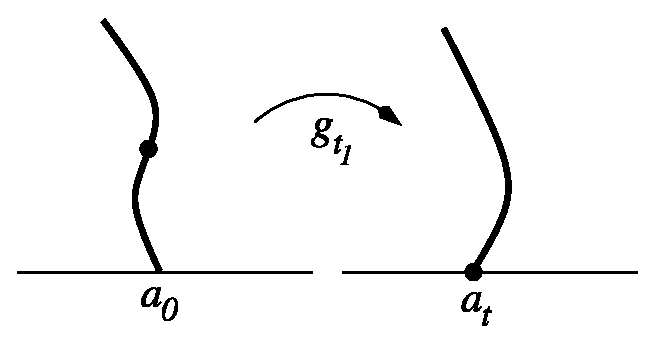
\includegraphics[width=60mm]{loewner}
    \caption{Конформное отображение $g_{t}(z):\mathbb{H}_{t}\to \mathbb{H}$.}}
  \label{fig:sle2}
\end{figure}

В статье \cite{schramm2000scaling} было показано, что  $g_{t}(z)$ удовлетворяет стохастическому дифференциальному уравнению
\begin{equation}
\label{eq:166}
  \frac{\partial g_t(z)}{\partial t} = \frac{ 2}{g_t(z)-\sqrt{\kappa}\xi_{t}} ,
\end{equation}
здесь $\xi_{t}$ -- Броуновское движение. Динамика конца  $z_{t}$ критической кривой $\gamma_{t}$ (конец следа эволюции Шрамма-Левнера) описывается уравнением $z_{t}=g_{t}^{-1}(\sqrt{\kappa}\xi_{t})$. 

Стохастический процесс, который удовлетворяет уравнению \eqref{eq:166} называется {\it эволюцией Шрамма-Левнера} на верхней полуплоскости $\mathbb{H}$. Для нас будет удобнее использовать отображение $w_{t} (z)=g_{t}(z)-\sqrt{\kappa}\xi_{t}$, так что уравнение \eqref{eq:166} переписывается в виде
\begin{equation}
  \label{eq:120}
       d w _{t}= \frac{2dt}{w_{t} }-\sqrt{\kappa}\xi_{t}  
\end{equation}
Эволюция Шрамма-Левнера порождает конформно-инвариантную вероятностную меру на кривых $\gamma_{t}$ в $\mathbb{H}$.

\subsection{Мартингалы эволюции Шрамма-Левнера и корреляционные функции в конформной теории поля}
\label{sec:corr-betw-sle}

Теперь рассмотрим наблюдаемые в присутствии следа эволюции Шрамма-Левнера. Математическое ожидание решеточной наблюдаемой $\mathcal{O}$ на верхней полуплоскости можно вычислить как сумму ожиданий этой наблюдаемой в присутствии (конечной части) траектории эволюции Шрамма-Левнера  $\gamma_{t}$ вплоть до некоторого времени $t$, умноженных на вероятность этой траектории:
\begin{equation*}
  \prec \mathcal{O} \succ_{\mathbb{H}}=\mathbb{E}\left[\prec\mathcal{O}\succ_{\gamma_{t}}\right]=\sum_{\gamma_{t}} P\left[C_{\gamma_{t}}\right] \prec \mathcal{O} \succ_{\gamma_{t}}
\end{equation*}
Решеточная наблюдаемая  $\prec \mathcal{O} \succ_{\mathbb{H}}$ не зависит от  $t$, следовательно $\prec\mathcal{O}\succ_{\gamma_{t}}$ -- мартингал.

В непрерывном пределе решеточные наблюдаемые сходятся к корреляционным функциям в конформной теории поля \cite{bauer2003sle,bauer2003conformal,bauer2002sle}. Мы должны учесть изменение граничных условий на конце следа эволюции Шрамма-Левнера и на бесконечности, так что соотношение имеет вид:
\begin{equation}
  \prec \mathcal{O} \succ_{\mathbb{H}_{t}}\to \mathcal{F}(\left\{z_{i}\right\})_{\mathbb{H}_{t}}=
  \frac{\left< \mathcal{O}(\{z_{i}\})\phi(z_{t})\phi^{\dagger}(\infty)\right>_{\mathbb{H}_{t}}}{\left<\phi(z_{t})\phi^{\dagger}(\infty)\right>_{\mathbb{H}_{t}}}
%% =
%%   \frac{\left<^{g_{t}}
%% \mathcal{O}\phi(\xi_{t})\phi^{\dagger}(\infty)\right>_{\mathbb{H}}}{\left<\phi(\xi_{t})\phi^{\dagger}(\infty)\right>_{\mathbb{H}}}
\label{eq:162}
\end{equation}

%% Here $\phi(z_{t})$ is a primary field corresponding to boundary condition changing operator.
%% We've used the conformal map $g_{t}$ to get the expression on the whole plane in equation \eqref{eq:162}.
Мы рассматриваем теорию с границей, так что мы должны использовать модели граничной конформной теории поля и накладывать соответствующие граничные условия \cite{cardy1984conformal,cardy1989boundary,cardy1991bulk}. В случае верхней полуплоскости корреляционные функции в граничной конформной теории поля могут быть переписаны как корреляционные функции для теории на всей плоскости, но с удвоенным числом полей (см. раздел \ref{sec:boundary-cft}).

% Here we are interested mainly in properties of boundary condition changing operator $\phi$. 

Мы предполагаем, что $\mathcal{F}$ содержит некоторый набор примарных полей  $\varphi_{i}$ с конформными весами $h_{i}$. Так как мы рассматриваем граничную конформную теорию поля, мы должны добавить объемные поля в сопряженных точках  $\bar z_{i}$.  Кроме того, у нас есть операторы смены граничного условия   $\phi$ на конце следа эволюции Шрамма-Левнера и на бесконечности. Воспользуемся конформным отображением   $w(z):\mathbb{H}\setminus\gamma_{t}\to \mathbb{H}$, чтобы переписать выражение \eqref{eq:162} на верхней полуплоскости без разреза:
\begin{equation}
  \mathcal{F}(\left\{z_{i}\right\})_{\mathbb{H}_{t}}=\prod \left(\frac{\partial w(z_{i})}{\partial z_{i}}\right)^{h_{\lambda_i}} 
  \prod \left(\frac{\partial \bar w(\bar z_{i})}{\partial \bar z_{i}}\right)^{h_{\lambda^{*}_i}}
  \mathcal{F}(\left\{w_{i}, \bar w_{i}\right\})_{\mathbb{H}}
  \label{eq:69}
\end{equation}

Теперь нам нужно рассмотреть, как преобразуется конец следа эволюции Шрамма-Левнера  $\gamma_{t}$ при переходе от времени $t$ к $t+ dt$. Первый множитель в правой части уравнения  (\ref{eq:69}) дает нам
\begin{equation*}
  -\frac{2h_{\lambda_{i}}}{w_{i}^{2}}\left(\frac{\partial w_{i}}{\partial z_{i}}\right)^{h_{i}}.
\end{equation*}
Для преобразования примарных полей  $\varphi_{\lambda_{i}}$ имеет место равенство
\begin{equation}
\label{eq:70}
  d\varphi_{i}(w_{i}) = \mathcal{G}_{i}\varphi_{i}(w_{i})=\left(\frac{2dt}{w_{i}}-\sqrt{\kappa} d\xi_{t}\right) \partial_{w_{i}}\varphi_{i}(w_{i}) 
\end{equation}
Мы обозначим генератор этого преобразования через  $\mathcal{G}_{i}$.

Так как $ \prec\mathcal{O}\succ_{\gamma_{t}}$ --  мартингал, математическое ожидание его приращения при эволюции от  $t$ к $t+dt$ равняется нулю
\begin{equation}
  \mathbb{E}\left[\prec\mathcal{O}\succ_{\gamma_{t}}\right]=    \mathbb{E}\left[\prec\mathcal{O}\succ_{\gamma_{t+dt}}\right], \quad d\mathbb{E}\left[ \prec\mathcal{O}\succ_{\gamma_{t}}\right]=0
\label{eq:163}
\end{equation}
Используем исчисление Ито и получим выражение для дифференциала $\mathcal{F}$:
\begin{equation}
d \mathcal{F}_{\mathbb{H}_{t}}= \left(\prod_{i=1}^{2N}\left(\frac{\partial w_{i}}{\partial z_{i}}\right)^{h_{i}}\right)\left(-\sum_{i=1}^{2N}\frac{2h_{i}dt}{w_{i}^{2}}+\left[\sum_{i=1}^{2N}\mathcal{G}_{i}+\frac{1}{2}
      \sum_{i,j}\mathcal{G}_{i}\mathcal{G}_{j}\right]\right)\mathcal{F}_{\mathbb{H}}=0
\label{eq:150}
\end{equation}
Подставим формулу \eqref{eq:70} и получим уравнение
\begin{equation}
  \left( \sum_{i}\left[-\frac{2h_{i}}{w_{i}^{2}} +\frac{2}{w_{i}}\partial_{w_{i}}\right]+\frac{\kappa}{2}\sum_{i,j}\partial_{w_{i}} \partial_{w_{j}}\right)\mathcal{F}(\left\{z_{i}\right\})=0
\label{eq:165}
\end{equation}

Для корреляционных функций вторичных полей  $L_{-n}\phi$ имеет место уравнение
\begin{equation}
\left< (L_{-n}\phi)(z) \varphi_{1}\dots \varphi_{N}\right>=\mathcal{L}_{-n}\left<\phi\varphi_{1}\dots\varphi_{N}\right>,
\end{equation}
где $n\geq 1$ и
\begin{equation*}
  \mathcal{L}_{-n}=\sum_{i=1}^{N} \left(\frac{(n-1)h_{i}}{(w_{i}-z)^{n}} -\frac{1}{(w_{i}-z)^{n-1}}\partial_{w_{i}}\right)
\end{equation*}
(См. \cite{difrancesco1997cft}). То есть мы можем переписать дифференциальное уравнение \eqref{eq:165} как алгебраическое уравнение на поле $\phi$, соответствующее оператору смены граничных условий:
\begin{equation}
  \label{eq:168}
   \left<\left([L_{-2}-\frac{\kappa}{2}L_{-1}^{2}]\phi\right)(0)\; \varphi_{1}\dots \varphi_{2N}\right>=0.
\end{equation}
В случае минимальных моделей набор примарных полей конечен и все состояния можно получить через соответствие между полями и состояниями
\cite{belavin1984ics}, \cite{difrancesco1997cft}. 
Равенство \eqref{eq:168} верно для произвольной наблюдаемой $\mathcal{O}$ и для произвольных примарных поле $\varphi_{i}$, так что $\psi=[L_{-2}-\frac{\kappa}{2}L_{-1}^{2}]\phi$ -- нулевое поле уровня два и $\psi(0)\left|0\right>$ -- нулевое состояние уровня два. В минимальных унитарных моделях существует только два примарных поля, порождающих модули Верма алгебры Вирасоро с нулевыми состояниями на уровне два. Это поля $\phi_{1,2}$ и $\phi_{2,1}$, так что $\phi\sim \phi_{1,2} \;\text{или}\; \phi_{2,1}$. 

\subsection{Модели Весса-Зумино-Новикова-Виттена и эволюция Шрамма-Левнера}
\label{sec:sle-wzw-models}
Чтобы обобщить анализ предыдущего раздела  \ref{sec:corr-betw-sle} на не-минимальные модели мы должны принять во внимание дополнительные симметрии. Модели Весса-Зумино-Новикова-Виттена обладают симметрией Каца-Муди в дополнение к конформной инвариантности, приводящей к появлению алгебры Вирасоро. Мы описали ВЗНВ-модели в разделе \ref{sec:WZNW-models}. 

Рассмотрим эволюцию Шрамма-Левнера в ВЗНВ-моделях. 
Подобно минимальным моделям мы рассматриваем наблюдаемые
\begin{equation*}
  \mathcal{F}(\left\{z_{i}\right\})_{\mathbb{H}_{t}}=
  \frac{\left<\phi_{\Lambda}(z_{t}) \varphi_{\lambda_1}(z_{1}) \dots \varphi_{\lambda_n}(z_{n}) \varphi_{\lambda^{*}_1}(\bar z_{1}) \dots \varphi_{\lambda^{*}_n}(\bar z_{n})
      \phi_{\Lambda^{*}}(\infty)\right>}{\left<\phi_{\Lambda}(z_{t})\phi_{\Lambda^{*}}(\infty)\right>},
\end{equation*}
где примарные объемные поля нумеруются весами $\lambda_i$.

Мы опять используем конформное отображение  $w(z):\mathbb{H}\setminus\gamma_{t}\to \mathbb{H}$ чтобы переписать формулу для наблюдаемых на всей верхней полуплоскости.
\begin{equation}
  \mathcal{F}(\left\{z_{i}\right\})_{\mathbb{H}_{t}}=\prod \left(\frac{\partial w(z_{i})}{\partial z_{i}}\right)^{h_{\lambda_i}} 
  \prod \left(\frac{\partial \bar w(\bar z_{i})}{\partial \bar z_{i}}\right)^{h_{\lambda^{*}_i}}
  \mathcal{F}(\left\{w_{i}, \bar w_{i}\right\})_{\mathbb{H}}
  \label{eq:177}
\end{equation}

В результате эволюции от $t$ к $t+dt$ первый множитель дает нам $-\frac{2h_{\lambda_{i}}}{w_{i}^{2}}\left(\frac{\partial w_{i}}{\partial z_{i}}\right)^{h_{\lambda_{i}}}$.

При рассмотрении полей нам нужно добавить случайное калибровочное преобразование  (случайное блуждание в $G$) к стохастическому процессу \cite{bettelheim2005stochastic}, \cite{alekseev2010sle}. 
Для полей мы имеем
\begin{equation*}
  d\varphi_{\lambda_{i}}(w_{i}) = \mathcal{G}_{i}\varphi_{\lambda_{i}}(w_{i}),
\end{equation*}
так что в генераторе преобразования поля появляется дополнительный член
\begin{equation}
  \mathcal{G}_{i}=\left(\frac{2dt}{w_{i}}-\sqrt{\kappa} d\xi_{t}\right) \partial_{w_{i}}+\frac{\sqrt{\tau}}{w_{i}}\sum_{a=1}^{\mathrm{dim} \gf}\left(d \theta ^{a} t^{a}_{i}\right)
\label{eq:159}
\end{equation}
Здесь  $d\theta^{a}$ -- генераторы  $\mathrm{dim}\gf$--мерного Броуновского движения, с $\mathbb{E}[d\theta^{a}d\theta^{b}]=\delta_{ab}dt$. Мы предполагаем, что $t^{a}$ -- это базис в $\gf$, ортогональный по отношению к форме Киллинга $\mathcal{K}$, $\mathcal{K}(t^{a},t^{b})=\delta_{ab}$.

Воспользуемся формулой \eqref{eq:150} и получим следующее уравнение из условий для мартингала:
\begin{equation}
  \left(-2 \mathcal{L}_{-2}+\frac{1}{2}\kappa \mathcal{L}_{-1}^{2}+\frac{1}{2}\tau\sum_{a} \mathcal{J}^{a}_{-1} \mathcal{J}^{a}_{-1}\right)        \mathcal{F}(\left\{w_{i}, \bar w_{i}\right\})_{\mathbb{H}}=0,
  \label{eq:167}
\end{equation}
где
\begin{equation*}
  \mathcal{L}_{-n}=\sum_{i}\left(\frac{(n-1)h_{\lambda_{i}}}{(w_{i}-z)^{n}}-\frac{1}{(w_{i}-z)^{n-1}}\partial_{w_{i}}\right);\quad \mathcal{J}^{a}_{{-n}}=-\sum_{i}\frac{t^{a}_{i}}{(w_{i}-z)^{n}}
\end{equation*}
Мы снова перепишем уравнение в виде алгебраического соотношения на поле, соответствующее оператору смены граничного условия. Теперь
\begin{equation}
  \left| \psi\right>=\left(-2 L_{-2}+\frac{1}{2}\kappa L_{-1}^{2}+\frac{1}{2}\tau\sum_{a} J^{a}_{-1} J^{a}_{-1}\right) \left|\phi_{\Lambda}\right>    
  \label{eq:16}
\end{equation}
является нулевым состоянием уровня два.
Из того, что корреляторы примарных полей с полем $\psi$ равны нулю следует, что состояние $\left|\psi\right>$ содержится в инвариантном подмодуле модуля Верма аффинной алгебры $\gfh$, порожденного действием операторов $J^a_n$ на состояние $\phi_{\Lambda}$, отвечающее старшему весу $\Lambda$. Таким образом, условие мартингала относительно эволюции Шрамма-Левнера эквивалентно тому, что некоторый вектор не принадлежит неприводимому модулю аффинной алгебры, а содержится в максимальном инвариантном подмодуле модуля Верма. Как видно, например, из конструкции БГГ-резольвенты (см. главу \ref{cha:BGG}), инвариантные подмодули в модуле Верма тесно связаны со структурой сингулярного элемента неприводимого модуля. 

Если на состояние $\left|\psi\right>$ подействовать повышающими операторами, мы должны получить ноль.
\begin{eqnarray}
 \label{eq:34}
 L_{1}\left|\psi\right>=0\\
  L_{2}\left|\psi\right>=0
\end{eqnarray}
В силу конструкции Сугавары (\ref{eq:91}) $  L_n=\frac{1}{2(k+h^{\vee})}\sum_a\sum_m:J^a_m J^a_{n-m}:$ это условие может быть выполнено только если $J^{a}_{n} \left|\psi\right>=0$
\begin{eqnarray}
  \label{eq:36} 
  J^{a}_{1} \left|\psi\right>=0\\
  J^{a}_{2}\left|\psi\right>=0.
\end{eqnarray}
Эти уравнения можно переписать как алгебраические соотношения, связывающие параметры случайного блуждания $\kappa, \tau$ с уровнем  $k$ представления аффинной алгебры Ли, если воспользоваться коммутационными соотношениями  (\ref{eq:102}), (\ref{eq:90}). Полный анализ таких алгебраических соотношений проведен в работе \cite{alekseev2010sle}.

Мы продемонстрируем другой подход к анализу соотношения (\ref{eq:16}). С точки зрения конечномерной подалгебры $\gf\subset\gfh$ все три слагаемых, действующих на состояние $\left|\phi_{\Lambda}\right>$ в формуле (\ref{eq:16}), являются квадратичными операторами Казимира (пропорциональны $\sum_a J^a J^a$). Поэтому состояние $\left|\psi\right>$ отвечает весу $\Lambda-2\delta$. 

Из этого следует необходимое условие на уровень и старший вес $\Lambda$: вектор веса  $\Lambda-2\delta$ должен содержаться в модуле Верма $V^{\mu}_{\gfh}$, старший вес которого $\mu=w(\Lambda+\rho)-\rho$ является сингулярным для неприводимого модуля $L^{\Lambda}_{\gfh}$. То есть должны существовать неотрицательные числа $a_0,\dots,a_r\in \mathbb{Z}_+$ ($r=\mathrm{rank}(\gf)$)  такие, что 
\begin{equation}
  \Lambda-2\delta = \mu-\sum_{k=0}^r a_k \alpha_k.
\label{eq:109}
\end{equation} 
Рассмотрим сингулярные веса с минимальным грейдом, которые могут входить в правую часть уравнения (\ref{eq:109}).
Во-первых, это сингулярные веса в нулевом грейде, которые совпадают с сингулярными весами неприводимого модуля $L^{\Lambda}$ конечномерной алгебры $\gf$.
Так как $\alpha_0 = \delta-\theta$ получаем в этом случае, что $a_0=2$ и $\Lambda-\mu= 2\theta-\sum_{k=1}^r a_k \alpha_k, \; a_k\geq 0$. В случае алгебры $\gf=\mathfrak{su}(2)$ имеем $\Lambda=l\omega_1,\; \theta=2\omega_1,\; \rho=\omega_1,\; \mu=-(l+2)\omega_1$ и $2l+2=4-2a_1$. То есть $a_1=0$ и $l=1$, а поле $\phi_{\Lambda}$ имеет спин $\frac{1}{2}$. В случае алгебры $\gf=\mathfrak{su}(N)$ аналогичное рассуждение выполняется для каждого из индексов Дынкина, отличных от нуля. То есть равенство (\ref{eq:109}) может выполняться только если каждый из индексов Дынкина не более единицы. 

Вспомним, что группа Вейля аффинной алгебры Ли $\gfh$  представляет собой полупрямое произведение группы Вейля конечномерной алгебры $\gf$ и группы трансляций $T=\left\{t_{\alpha_k}\right\}$, порожденной простыми корнями $\alpha_1,\dots,\alpha_r$. Так как  $t_{\alpha}\lambda=\lambda+\frac{2(\lambda,\delta)}{(\alpha,\alpha)}\alpha-\left(\frac{(\alpha,\alpha)}{2} (\lambda,\delta)+(\lambda,\alpha)\right) \delta$, в случае длинного корня $\alpha:\; (\alpha,\alpha)=2$ при $k>2$ и $(\alpha,\lambda)\neq 0$ условие (\ref{eq:109}) не может выполняться для $\mu=t_{\alpha} w(\Lambda+\rho)-\rho, \; w\in W_{\gf}$ просто в силу того, что грейд в правой части меньше $-2$. 

Таким образом условие (\ref{eq:109}), характеризующее структуру сингулярного элемента представления аффинной алгебры Ли $\gfh$, исключает из рассмотрение большое количество примарных полей $\phi_{\Lambda}$. Вместе с тем это условие несколько слабее, чем необходимые условия, полученные в разделе 2 работы \cite{alekseev2010sle}. 


\subsection{Coset-модели и эволюция Шрамма-Левнера}
\label{sec:coset-models-sle}
Теперь мы обобщим анализ соответствия между эволюцией Шрамма-Левнера и конформной теорией поля на случай coset-моделей \cite{Goddard198588}. Такие модели задаются алгеброй Ли $\gf$ и ее подалгеброй $\af$. Воспользуемся обозначениями, введенными в разделе \ref{sec:coset-models-cft}.

Как мы упоминали в главе \ref{cha:CFT}, $G/A$-coset модель конформной теории поля может быть реализована как ВЗНВ-модель (с калибровочной группой $G$), взаимодействующая с чисто калибровочными полями, с калибровочной группой $A\subset G$ \cite{gawdzki1988g,figueroa89equivalence}. Как было показано в главе \ref{cha:CFT}, действие записывается через поля  $g:\mathbb{C}\to G$ и $A,\bar A:\mathbb{C}\to \af$ (\ref{eq:38}). Здесь $\af$ -- алгебра Ли, соответствующая группе Ли $A$.

Если мы фиксируем  $A$-калибровку, у нас останется  $G/A$ калибровочная инвариантность. Значит мы должны добавить случайные калибровочные преобразования к эволюции Шрамма-Левнера, аналогично случаю ВЗНВ-моделей из предыдущего раздела (См. также \cite{bettelheim2005stochastic}).  Обозначим через $t^{a}_{i}$ ($\tilde{t}^{b}_{i}$) генераторы представления алгебры $\gf$ (соответственно, представления $\af$), соответствующего примарному полю $\varphi_{i}$.

Рассмотрим эволюцию следа SLE $\gamma_{t}$ с момента   $t$ до $t+ dt$.  Первый сомножитель в правой части уравнения (\ref{eq:177}) дает нам
\begin{equation*}
  -\frac{2h_{i}}{w_{i}^{2}}\left(\frac{\partial w_{i}}{\partial z_{i}}\right)^{h_{i}}.
\end{equation*}
Напомним, что через  $\mathcal{G}_{i}$ мы обозначили  генераторы инфинитезимальных преобразований примарных $\varphi_{i}$:$d\varphi_{i}(w_{i}) = \mathcal{G}_{i}\varphi_{i}(w_{i})$. Нормируем дополнительное $\left(\dim\gf\right)$-мерное Броуновское движение следующим образом: $\mathbb  {E}\left[d\theta^{a}\; d\theta^{b}\right]=\mathcal{K}(t^{a},t^{b})dt$. Тогда генератор преобразования поля равен
\begin{equation}
  \mathcal{G}_{i}=\left(\frac{2dt}{w_{i}}-\sqrt{\kappa} d\xi_{t}\right) \partial_{w_{i}}+\frac{\sqrt{\tau}}{w_{i}}\left(\sum_{a:\mathcal{K}(t^{a},\tilde{t}^{b})=0}\left(d \theta ^{a} t^{a}_{i}\right)\right).
\label{eq:179}
\end{equation}
То есть мы фиксировали  $A$-калибровку, разрешив случайное блуждание только в направлении, ортогональном подалгебре $\af$. 

Формула Ито дает нам выражение для дифференциала $\mathcal{F}$, который равняется нулю в силу условия мартингала:
\begin{multline}
d \mathcal{F}_{\mathbb{H}_{t}}= \left(\prod_{i=1}^{2N}\left(\frac{\partial w_{i}}{\partial z_{i}}\right)^{h_{i}}\right)
\left(-\sum_{i=1}^{2N}\frac{2h_{i}dt}{w_{i}^{2}}+\left[\sum_{i=1}^{2N}\mathcal{G}_{i}+\frac{1}{2}
      \sum_{i,j}\mathcal{G}_{i}\mathcal{G}_{j}\right]\right)\mathcal{F}_{\mathbb{H}}\\=0
\label{eq:180}
\end{multline}
Подставляя определение \eqref{eq:179}, мы получаем
\begin{equation}
  \left(-2 \mathcal{L}_{-2}+\frac{1}{2}\kappa \mathcal{L}_{-1}^{2}+\frac{\tau}{2}\left( \sum_{a} \mathcal{J}^{a}_{-1} \mathcal{J}^{a}_{-1}-
      \sum_{b}\tilde{\mathcal{J}}^{b}_{-1} \tilde{\mathcal{J}}^{b}_{-1}\right)\right)        \mathcal{F}_{\mathbb{H}}=0,
\label{eq:181}
\end{equation}
где
\begin{eqnarray*}
  \mathcal{L}_{-n}=\sum_{i}\left(\frac{(n-1)h_{i}}{(w_{i}-z)^{n}}-\frac{\partial_{w_{i}}}{(w_{i}-z)^{n-1}}\right),\\ \mathcal{J}^{a}_{{-n}}=-\sum_{i}\frac{t^{a}_{i}}{(w_{i}-z)^{n}};\; \tilde{\mathcal{J}}^{b}_{{-n}}=-\sum_{i}\frac{\tilde{t}^{b}_{i}}{(w_{i}-z)^{n}}.
\end{eqnarray*}
Это равенство эквивалентно следующему алгебраическому условию на граничное состояние $\phi(0)\left|0\right>$:
\begin{multline}
\label{eq:182}
  \left<0\left|\phi(\infty)\varphi_{1}(w_{1})\dots\varphi_{2N}(w_{2N})\right.\right.\\
  \left(-2L_{-2}+\frac{1}{2}\kappa L_{-1}^{2}+\frac{1}{2}\tau \left(\sum_{a=1}^{\dim\gf}J^{a}_{-1}J^{a}_{-1}-\sum_{b=1}^{\dim\af}\tilde{J}^{b}_{-1}\tilde{J}^{b}_{-1}\right)\right)\\
\left.\phi(0)|0\right>=0.
\end{multline}
Так как набор  $\{\phi_{i}\}$ состоит из произвольных примарных полей, мы заключаем, что 
\begin{multline}
\label{eq:126}
|\psi>=\left(-2L_{-2}+\frac{1}{2}\kappa L_{-1}^{2}+\frac{1}{2}\tau \left(\sum_{a=1}^{\dim\gf}J^{a}_{-1}J^{a}_{-1}-\sum_{b=1}^{\dim\af}\tilde{J}^{b}_{-1}\tilde{J}^{b}_{-1}\right)\right)
\cdot\phi(0)|0>
\end{multline}
является нулевым состоянием. Теперь мы можем подействовать на  $\psi$ повышающими операторами и получить уравнения на  $\kappa,\tau$. Так как в  coset-моделях коммутационные соотношения полной киральной алгебры даются выражением (\ref{eq:183}), для нас более удобно действовать операторами $L_{2}^{\gf}$ и $\left(L_{1}^{\gf}\right)^{2}$. 
Применение оператора $L_{2}^{\gf}$ дает
\begin{equation*}
  L_{2}^{\gf}\psi= \left(-8 L_{0}-c+ 3 \kappa L_{0}+\frac{1}{2}\tau (k \dim\gf-x_{e}k\dim\af)\right) \varphi_{(\mu,\nu)}=0
\end{equation*}
Здесь мы воспользовались тем, что $L_{0} \varphi_{(\mu,\nu)}=h_{(\mu,\nu)} \varphi_{(\mu,\nu)}$, с конформным весом  $h_{(\mu,\nu)}= \left(\frac{(\mu,\mu+2\rho)}{2(k+h^{\vee}_{\gf})}-\frac{(\nu,\nu+2\rho_{\af})}{2(k x_{e}+h^{\vee}_{\af})}\right)$, а центральный заряд равен $c=\frac{k\dim \gf}{k+h^{\vee}_{\gf}}-\frac{x_{e}k\dim \af}{x_{e} k+h^{\vee}_{\af}}$. В результате получаем соотношение на $\kappa,\tau$:
\begin{equation}
 (3\kappa-8)h_{(\mu,\nu)}-c+\tau (k\dim\gf-x_{e}k\dim\af) =0.
 \label{eq:184}
\end{equation}
Второе уравнение получается в результате действия $L_{1}^{\gf}$:
\begin{equation}
\label{eq:185}
 -12 h_{(\mu,\nu)}+2\kappa h_{(\mu,\nu)} (2h_{(\mu,\nu)}+1) + \tau
(C_{\mu}-\tilde{C}_{\nu})=0,
\end{equation}
здесь $C_{\mu}=(\mu,\mu+2\rho)$ и $\tilde{C}_{\nu}=(\nu,\nu+2\rho_{\af})$ -- это собственные значения квадратичных операторов Казимира $\sum_{a}t^{a}t^{a}$ и $\sum_{b}\tilde{t}^{b}\tilde{t}^{b}$ алгебр Ли $\gf$ и $\af$.
Равенства \eqref{eq:183},\eqref{eq:185} представляют собой необходимые условия того, чтобы корреляционные функции в coset-модели конформной теории поля являлись мартингалами по отношению к эволюции Шрамма-Левнера. 

Из уравнения  \eqref{eq:183},\eqref{eq:185} мы сразу получаем значения  $\kappa,\tau$ для каждой пары весов $(\mu,\nu)$ алгебр $\gf$ и $\af$. 

\subsubsection{Примеры}
\label{sec:examples-1}


Рассмотрим простой пример.Пусть $G=SU(2)$ и $A=U(1)$, соответствующая алгебра Ли $\gf=\mathrm{su}(2)$ имеет генераторы $J^{1},J^{2},J^{3}$, а $\af=\mathrm{u}(1)$ -- генератор $J^{3}$, $\af\subset\gf$.  Заметим, что $\mathcal{K}(J^{a},J^{b})=2\delta^{ab}$. Как известно,  $\frac{\hat{su}(2)_{N}}{\hat{u}(1)_{N}}$-coset модель эквивалентна  $Z_{N}$-парафермионам \cite{difrancesco1997cft}.
%%We label weights by Dynkin labels, so $J^{3}_{0}\phi_{(\mu,\nu)}=\frac{\mu}{2} \phi_{(\mu,\nu)}$.
Примарные поля нумеруются парами весов $(\mu,\nu)$, которые мы будем задавать индексами Дынкина $(k,l)$. 

Уравнение \eqref{eq:126} теперь имеет вид
\begin{equation}
  \label{eq:138}
  \psi=\left(-2L_{-2}+\frac{1}{2}\kappa L_{-1}^{2}+\frac{1}{2}\tau \left(J^{1}_{-1}J^{1}_{-1}+J^{2}_{-1}J^{2}_{-1}\right)\right) \phi_{(\mu,\nu)}
\end{equation}
Если перейти к базису $J^{+}=\frac{J^{1}+iJ^{2}}{\sqrt{2}},\; J^{-}=\frac{J^{1}-iJ^{2}}{\sqrt{2}}$, это уравнение будет переписано в виде
\begin{equation}
 \psi= \left(-2 L_{-2}+\frac{\kappa}{2}L_{-1}^{2}+\frac{\tau}{2}\left[J^{+}_{-1}J^{-}_{-1}+J^{-}_{-1}J^{+}_{-1}\right]\right) \phi_{(\mu,\nu)},
\label{eq:140}
\end{equation}
аналогичном уравнениям для парафермионных полей, выведенным в статье  \cite{santachiara2008sle}.

В данном примере центральный заряд равен
\begin{equation}
  \label{eq:160}
  c=\frac{3N}{N+2}-1=\frac{2N-2}{N+2},
\end{equation}
а конформный вес примарного поля с весами, заданными индексами Дынкина $(k,l)$,  равен $h_{(k,l)}=\frac{k(k+2)}{4(N+2)}-\frac{l^{2}}{4N}$.

Случай  $N=2$, $c=\frac{1}{2}$ соответствует модели Изинга. В этом случае у нас есть два нетривиальных примарных поля с конформными весами $h_{(2,0)}=1/2, h_{(1,1)}=1/16$. Подставляя поле $\varphi_{(2,0)}$ в выражения (\ref{eq:183},\ref{eq:185}) мы получаем уравнения: $3\kappa-9+4\tau =0;\quad -3+\kappa+4\tau=0$ с решением $\kappa=3, \tau=0$. Для поля  $\varphi_{(1,1)}$ получаются соотношения $3\kappa-16+64\tau=0,\quad -64+9\kappa + 64\tau=0$ и значения параметров $\kappa=16/3, \tau=0$. То есть в случае модели Изинга нет необходимости в дополнительном случайном блуждании, а значения параметра эволюции Шрамма-Лёвнера $\kappa$ совпадают с известными результатами \cite{schramm2006conformally}.

При  $N=3$ центральный заряд парафермионной модели равен $c=\frac{4}{5}$. Конформные веса принимают значения $h_{(0,0)}=0$, $h_{(0,2)}=h_{(0,-2)}=\frac{2}{3}\; \mathrm{mod}\; 1$, $h_{(2,0)}=\frac{2}{5}$, $h_{(2,2)}=h_{(2,-2)}=\frac{1}{15}$.  Соответствующие значения параметров  $\kappa,\tau$ равны: $(\frac{208}{25},\frac{242}{225}), (\frac{10}{3},0),(\frac{80}{19},\frac{14}{171})$. Как было указано в работе \cite{santachiara2008sle}, поле  $\varphi_{(2,0)}$ с конформным весом  $h_{(2,0)}=\frac{2}{5}$ образует  $Z_{3}$-синглет, так что дополнительное случайное блуждание не возникает и  $\tau=0$. Вид уравнения (\ref{eq:182}) аналогичен полученному в работе \cite{santachiara2008sle} для парафермионов, но нормировка параметра $\tau$ отличается.

Легко видеть, что для реализации минимальных унитарных моделей в виде  $\frac{\hat{su}(2)_{N}\oplus \hat{su}(2)_{1}}{\hat{su}(2)_{N+1}}$-coset моделей с центральными зарядами $c=\frac{3N}{N+2}+1-\frac{3(N+1)}{N+3}=1-\frac{6}{(N+2)(N+3)}$ система уравнения (\ref{eq:183},\ref{eq:185}) всегда совместна при  $\tau=0$ и мы получаем стандартную для минимальных моделей связь между параметром эволюции Шрамма-Левнера $\kappa$ и центральным зарядом $c=\frac{(6-\kappa)(3\kappa-8)}{2\kappa}$.

\subsection{Coset-модели и интегрируемые деформации конформной теории поля}
\label{sec:outlook}


Связь между  ВЗНВ-моделями и эволюцией Шрамма-Левнера с дополнительным броуновским движением на групповом многообразии была установлена в работе    \cite{bettelheim2005stochastic}. Авторы этой работы поставили задачу установления связи между параметрами эволюции Шрамма-Лёвнера для мартингалов в ВЗНВ, coset  и минимальных моделях конформной теории поля. Мы воспользовались методом, предложенным в работе \cite{alekseev2010sle} чтобы получить необходимые условия на мартингалы. Этот метод позволил нам сравнить наши результаты с результатами для парафермионов из работ \cite{santachiara2008sle,picco2008numerical}.

Реализация минимальных моделей посредством  coset-конструкции полезна при рассмотрении теории, возмущенной внешним магнитным полем \cite{fateev1990conformal,eguchi1989deformations,hollowood1989rational}. Эта модель подтверждается экспериментальными данными недавней работы \cite{coldea2010quantum}. Соотношения между корреляционными функциями в  coset-модели и наблюдаемыми эволюции Шрамма-Лёвнера могут выступить стартовой точкой в изучении доменных стенок в решеточных моделях вдали от критической точки.

Массивные возмущения  $G/A$-coset модели могут быть реализованы как аффинная теория поля Тоды. Они классифицируются простыми корнями алгебры Ли $\gf$. Действие аффинной теории Тоды можно получить добавлением возмущающего члена в действие (\ref{eq:38}):
\begin{equation}
  S_{\text{pert}}=S_{G/A}(g,A,\bar A)-\frac{k\lambda}{2\pi}\int {\cal K} (g T, g^{-1} \bar T),
\end{equation}
где $T,\bar T\in \gf$ -- специальным образом выбранные элементы алгебры Ли \cite{bakas1996lagrangian,hollowood1995massive,park1994deformed}. Такое возмущение ведет к вставке некоторого примарного поля во все корреляторы \cite{hollowood1989rational}. Недавно было показано, что массивная эволюция Шрамма-Лёвнера вне критической точки содержит дополнительный член в движущем броуновском движении, который соответствует сносу \cite{makarov2010off,bauer2009off}. Необходимо проверить, что взаимодействие возмущающего примарного поля с  $\tau$-членом уравнения (\ref{eq:181}) приводит к такому же вкладу, что и введение массивного сноса в эволюцию Шрамма-Лёвнера. Кроме того, требуется сравнить массивные возмущения coset-моделей с результатами численного изучения доменных стенок в модели Изинга, возмущенной случайным гауссовым полем \cite{stevenson2011domain}.  

%%  
%%  \subsection{О связи мартингалов coset-моделей с классификацией операторов смены граничного условия}
%%  \label{sec:5-conclusion}
%%  
%%  Мы предложили способ обобщения эволюции Шрамма-Левнера для получения таких наблюдаемых, которые могут исследоваться методами конформной теории поля. Описание полей в coset-моделях нетривиально ввиду идентификации полей \cite{schellekens1990field} и необходимости в разрешении фиксированных точек \cite{Fuchs:1996dd,fuchs1996resolution}, которое не обсуждалась в данной главе. Эти тонкости могут усложнить решение уравнений  \eqref{eq:184}, \eqref{eq:185}. С другой стороны, использование уравнений Книжника-Замолодчикова  \cite{kogan1997knizhnik} для корреляционных функций в духе работы \cite{alekseev2010sle} приводит к матричным алгебраическим соотношениям, которые напоминают NIM-представления для граничных состояний \cite{ishikawa2003novel}. Дальнейшее изучение этого предмета может выявить глубокую алгебраическую связь условия мартингала с классификацией граничных состояний.
%%  

%%
%% End of file
%%% Local Variables: 
%%% mode: latex
%%% TeX-master: "thesis"
%%% End: 
